% Paquets généraux
\documentclass[a4paper,12pt,titlepage]{article}
\usepackage[T1]{fontenc}
\usepackage[utf8]{inputenc}
\usepackage[french]{babel}
\usepackage[gen]{eurosym}
%\usepackage[dvips]{graphicx}
\usepackage{fancyhdr}
\usepackage{pdfpages} 
\usepackage{multido}
\usepackage{hyperref}
%\usepackage{textcomp}
%\usepackage{aeguill}
\usepackage{schemabloc}
\usepackage[bitstream-charter]{mathdesign}
\usepackage{pstricks}
\usepackage{helvet}

\newcommand{\id}{71}
\newcommand{\nom}{Théorie des mécanismes}
\newcommand{\sequence}{04}
\newcommand{\nomsequence}{Liaisons entre les solides}
\newcommand{\num}{02}
\newcommand{\type}{KH}
\newcommand{\descrip}{Liaisons équivalentes, hyperstatisme, liaisons en série et en parallèle, théorie des graphes}
\newcommand{\competences}{B2-12: Proposer une modélisation des liaisons avec leurs caractéristiques géométriques. \\ &  B2-13: Proposer un modèle cinématique paramétré à partir d'un système réel, d'une maquette numérique ou d'u \\ &  B2-17: Simplifier un modèle de mécanisme. \\ &  B2-18: Modifier un modèle pour le rendre isostatique. \\ &  C1-04: Proposer une démarche permettant d'obtenir une loi entrée-sortie géométrique.  \\ &  C2-05: Caractériser le mouvement d'un repère par rapport à un autre repère. \\ &  C2-06: Déterminer les relations entre les grandeurs géométriques ou cinématiques. }
\newcommand{\nbcomp}{7}
\newcommand{\systemes}{}
\newcommand{\systemesnum}{}
\newcommand{\systemessansaccent}{}
\newcommand{\ilot}{2}
\newcommand{\ilotstr}{02}
\newcommand{\dossierilot}{\detokenize{Ilot_02 }}


\newcommand{\auteurun}{Renaud Costadoat}
\newcommand{\institute}{Lycée Dorian}


\usepackage{color}
\usepackage{xcolor}
\usepackage{colortbl}
\usepackage{helvet}
\renewcommand{\familydefault}{\sfdefault}
\usepackage{amsfonts}
\usepackage{amsmath}
%\usepackage{xspace}
\usepackage{varioref}
\usepackage{tabularx}
%\usepackage{floatflt}
\usepackage{graphics}
\usepackage{wrapfig}
\usepackage{textcomp}
\usepackage{tikz}
\usepackage{wrapfig}
\usepackage{gensymb}
\usepackage[european]{circuitikz}
\usetikzlibrary{babel}
\usepackage{ifthen}
\usepackage{cancel}
\usepackage{etoolbox}
\usepackage{multirow}
%\usepackage{boxedminipage}
\definecolor{gris25}{gray}{0.75}
\definecolor{bleu}{RGB}{18,33,98}
\definecolor{bleuf}{RGB}{42,94,171}
\definecolor{bleuc}{RGB}{231,239,247}
\definecolor{rougef}{RGB}{185,18,27}
\definecolor{rougec}{RGB}{255,188,204}%255,230,231
\definecolor{vertf}{RGB}{103,126,82}
\definecolor{vertc}{RGB}{220,255,191}
\definecolor{forestgreen}{rgb}{0.13,0.54,0.13}
\definecolor{blcr}{rgb}{0.59,0.69,0.84}
\definecolor{blfr}{rgb}{0.32,0.51,0.75}
\definecolor{orfr}{rgb}{0.90,0.42,0.15}
\definecolor{orcr}{rgb}{0.90,0.65,0.50}
\definecolor{orangef}{rgb}{0.659,0.269,0.072}
\definecolor{orange}{rgb}{0.58,0.35,0.063}
\definecolor{orangec}{rgb}{0.43,0.32,0.25}
\definecolor{rcorrect}{rgb}{0.6,0,0}
\definecolor{sequence}{rgb}{0.75,0.75,0.75}
\definecolor{competences}{rgb}{0.61,0.73,0.35}
\definecolor{grisf}{HTML}{222222}
\definecolor{grisc}{HTML}{636363}
\definecolor{normal}{HTML}{4087c4}
\definecolor{info}{HTML}{5bc0de}
\definecolor{success}{RGB}{92,184,92}
\definecolor{warning}{RGB}{240,173,78}
\definecolor{danger}{RGB}{217,83,79}
\hypersetup{                    % parametrage des hyperliens
    colorlinks=true,                % colorise les liens
    breaklinks=true,                % permet les retours à la ligne pour les liens trop longs
    urlcolor= blfr,                 % couleur des hyperliens
    linkcolor= orange,                % couleur des liens internes aux documents (index, figures, tableaux, equations,...)
    citecolor= forestgreen                % couleur des liens vers les references bibliographiques
    }

% Mise en page
\pagestyle{fancy}

\setlength{\hoffset}{-18pt}

\setlength{\oddsidemargin}{0pt} 	% Marge gauche sur pages impaire2s
\setlength{\evensidemargin}{0pt} 	% Marge gauche sur pages paires
\setlength{\marginparwidth}{00pt} 	% Largeur de note dans la marge
\setlength{\headwidth}{481pt} 	 	% Largeur de la zone de tête (17cm)
\setlength{\textwidth}{481pt} 	 	% Largeu\textbf{r de la zone de texte (17cm)
\setlength{\voffset}{-18pt} 		% Bon pour DOS
\setlength{\marginparsep}{7pt}	 	% Séparation de la marge
\setlength{\topmargin}{-30pt} 		% Pas de marge en haut
\setlength{\headheight}{55pt} 		% Haut de page
\setlength{\headsep}{20pt} 		% Entre le haut de page et le texte
\setlength{\footskip}{30pt} 		% Bas de\textbf{ page + séparation
\setlength{\textheight}{700pt} 		% Hauteur de l'icone zone de texte (25cm)
\setlength\fboxrule{1 pt}
\renewcommand{\baselinestretch}{1}
\setcounter{tocdepth}{1}
\newcommand{\cadre}[2]
{\fbox{
  \begin{minipage}{#1\linewidth}
   \begin{center}
    #2\\
   \end{center}
  \end{minipage}
 }
}


\newcommand{\titre}[1]
{\begin{center}
\cadre{0.8}{\huge #1} 
\end{center}
}

\newcounter{num_quest} \setcounter{num_quest}{0}
\newcounter{num_rep} \setcounter{num_rep}{0}

\newcommand{\question}[1]{\refstepcounter{num_quest}\par
~\ \\ \textbf{Question \arabic{num_quest} : }#1\label{q\the\value{num_quest}}\par
}

\newcommand{\reponse}[1]
{\noindent
\rule{\linewidth}{.5pt}\\
\textbf{Question \refstepcounter{num_rep}\ref{q\the\value{num_rep}} :} ~\ \\
#1}

% En tête et pied de page
\lhead{\nom}
\rhead{
\includegraphics[width=2cm]{../../img/logo}}
\lfoot{Renaud Costadoat}
\cfoot{Page \thepage}

\fancypagestyle{correction}{%
  \fancyhf{}
  \lhead{\colorbox{danger}{\begin{minipage}{0.65\paperwidth} \textcolor{white}{\textbf{Correction}} \end{minipage}} }
  \rhead{
\includegraphics[width=2cm]{../../img/logo}}
  \lfoot{Renaud Costadoat}
  \rfoot{\colorbox{danger}{\begin{minipage}{0.6\paperwidth} \begin{flushright}\textcolor{white}{\textbf{Correction}}\end{flushright} \end{minipage}} }}

\renewcommand{\footrulewidth}{0.4pt}

\usepackage{eso-pic}
\newcommand{\BackgroundPic}{%
\put(0,0){%
\parbox[b][\paperheight]{\paperwidth}{%
\vfill
\begin{center}
\hspace{0.5cm}\vspace{0.5cm}

\includegraphics[width=\paperwidth,height=\paperheight,%
keepaspectratio]{../../img/fond3}%
\end{center}
\vfill
}}}

\newcommand{\BackgroundPicdeux}{%
\put(25,-30){%
\parbox[b][\paperheight]{\paperwidth}{%
\vfill
\begin{center}
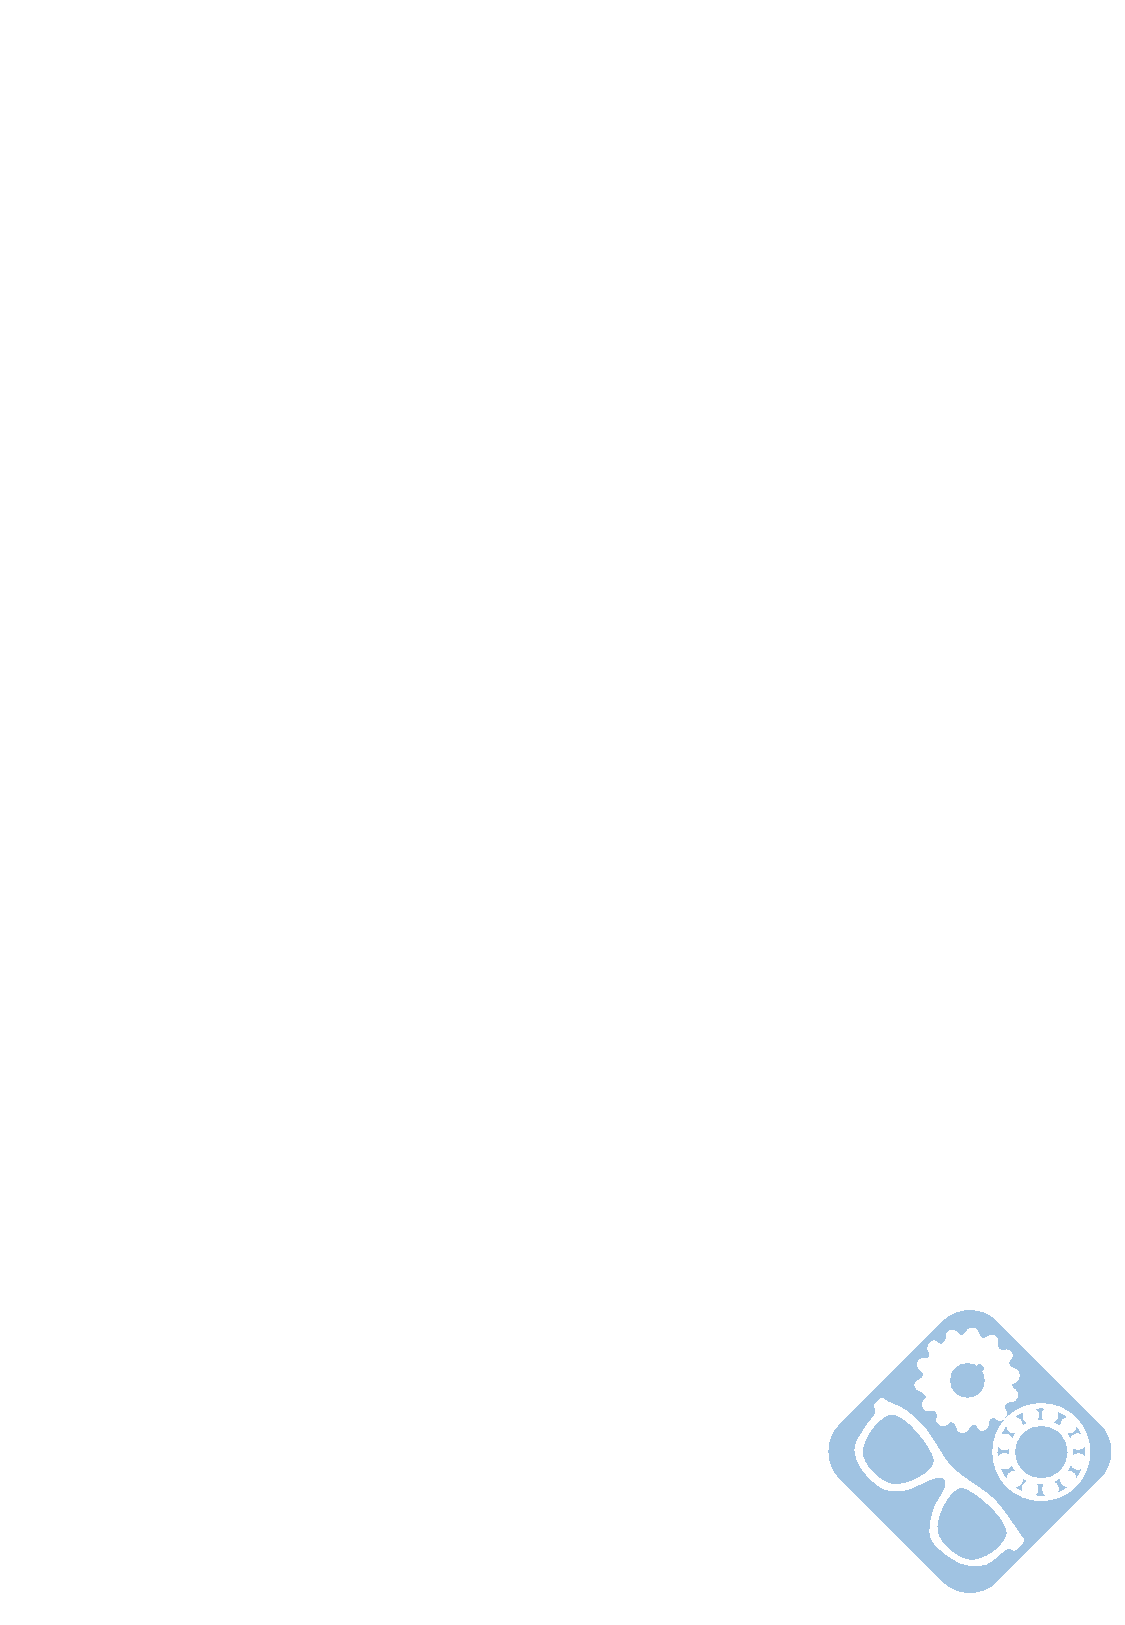
\includegraphics[width=\paperwidth,height=\paperheight,%
keepaspectratio]{../../img/fond4}%
\end{center}
\vfill
}}}

\begin{document}

\AddToShipoutPicture{\BackgroundPicdeux}

\pagestyle{fancy}

\section{Circuit RC}


%\subsection{Introduction}
%
%Définition de la transformation de Laplace :
%
%Soit f(t), une fonction de la variable temporelle réelle t et définie pour $t>0$. La transformée de Laplace de f(t), la fonction F(p), définie par l'intégrale généralisée :
%$F(p)=\int^{\infty}_0 e^{-pt}.f(t).dt$, notée $F(p)=L\left[f(t)\right]$
%
%p est la variable de Laplace, elle pet être une variable complexe ou réelle.
%
%\paragraph{Question 1:}
%
%Déterminer la transformée de Laplace de la fonction échelon u(t).
%
%\paragraph{Question 2:}
%
%Déterminer la transformée de Laplace de la fonction $g(t)=\frac{1}{T}.e^{\frac{-t}{T}}$.
%
%\paragraph{Question 3:}
%
%Déterminer l'antécédent de la fonction $F(p)=\frac{1}{p(1+Tp)}$ en décomposant F(p) en éléments simples. Tracer le graphe de l'original f(t) de F(p) pour $0<t<5T$.

\subsection{Présentation du système}

\begin{figure}[!h]
\begin{minipage}{.55\linewidth}
Un circuit RC est un circuit électrique, composé d'une résistance et d'un condensateur. Dans leur configuration série, les circuits RC permettent de réaliser des filtres électroniques passe-bas ou passe-haut.
\begin{center}
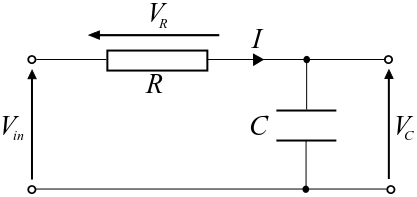
\includegraphics[width=0.8\linewidth]{img/Series-RC}
\caption{Circuit RC}
\label{fig:image1}
\end{center}
\end{minipage}
\hfill
\begin{minipage}{.40\linewidth}
\begin{center}
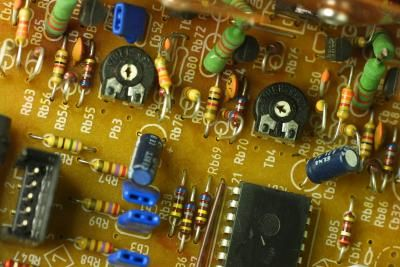
\includegraphics[width=0.8\linewidth]{img/circuit_RC.jpg}
\caption{Montage électronique}
\label{fig:image2}
\end{center}
Le système est modélisé par la figure \ref{fig:image1}. A t=0, le condensateur se charge.
\end{minipage}
\end{figure}

\paragraph{Question 1:}

Déterminer l'équation différentielle qui régit le système. L'entrée du système sera la tension V(t) et la sortie la tension aux bornes du condensateur. Les valeurs numériques sont les suivantes: $R=10\Omega$ et $C=1mF=10^{-3}F$.

\paragraph{Question 2:}

Résoudre cette équation à l'aide des transformées de Laplace. Déterminer l'expression de la sortie s(t) quand l'entrée e(t) est un échelon de valeur $E_0=2V$ et en faire la représentation graphique pour $0<t<0,05s$.

Déterminer l'écart statique $\epsilon_s=\lim\limits_{t \to +\infty}(e(t)-s(t))$ quand l'entrée e(t) est un échelon

\paragraph{Question 3:}

Déterminer $tr_{5\%}$, temps au bout duquel la sortie s(t) atteint 0,95 fois sa valeur à l'infini.

On présente à l'entrée une rampe de tension $e(t)=\alpha.t.u(t)$ où u(t) est la fonction échelon avec $\alpha=1V.s^{-1}$. On rappelle que : u(t)=0 pour $t<0$ et u(t)=1 pour $t>0$.

Déterminer l'expression de la sortie s(t) et établir sur le même graphe les représentations graphiques de s(t) et e(t).

Déterminer l'écart de traînage $\epsilon_v=\lim\limits_{t \to +\infty}(e(t)-s(t))$ quand l'entrée e(t) est une rampe.

\begin{center}
\begin{tabular}{|c|c||c|c|}
\hline
Temporel $f(t)$ & Laplace $F(p)$ & 
Temporel $f(t)$ & Laplace $F(p)$ \\
\hline
\hline
 &&& \\
Dirac $\delta(t)$ &
$F(p)=1$ &
Échelon $ u(t)=k $&
$ U(p) = \frac{k}{p}$
\\
&&& \\
\hline
&&& \\
$f(t) = t^n\cdot u(t)$ &
$F(p)=\frac{n!}{p^{n+1}} $ &
$\forall t\in ]0,t_1 [ \quad f(t)= A$ & 
$F(p) =A \cdot \frac{1-e^{-pt_1}}{p} $\\
&&& \\
\hline
&&& \\
$f(t) = \sin \left( \omega_0 t\right) \cdot u(t)$ &
$F(p) = \frac{\omega_0}{p^2+\omega_0^2} $ &
$f(t) = \cos \left( \omega_0 t\right) \cdot u(t)$ & 
$F(p) = \frac{p}{p^2+\omega_0^2} $ \\
&&& \\
\hline
&&& \\
$f(t)= e^{-at}\cdot u(t)$ & 
$F(p)= \frac{1}{p+a}$ &
$f(t) = e^{-at}\sin\left( \omega_0 t\right) \cdot u(t)$ &
$F(p)=\frac{\omega_0}{\left( p+a\right)^2 + \omega_0^2}$  \\
&&& \\
\hline
&&& \\
$f(t) = e^{-at}\cos\left( \omega_0 t\right) \cdot u(t)$ &
$F(p)=\frac{p+a}{\left( p+a\right)^2 + \omega_0^2}$  &
$f(t)=t^ne^{-at}u(t)$ & $F(p)=\frac{n!}{\left( p+a\right)^{n+1}}$ \\
&&& \\
\hline
\end{tabular}
\end{center}

\newpage

\section{Amortisseur}

%\subsection{Introduction}
%
%Définition de la transformation de Laplace :
%
%Soit f(t), une fonction de la variable temporelle réelle t et définie pour $t>0$. La transformée de Laplace de f(t), la fonction F(p), définie par l'intégrale généralisée :
%$F(p)=\int^{\infty}_0 e^{-pt}.f(t).dt$, notée $F(p)=L\left[f(t)\right]$
%
%p est la variable de Laplace, elle peut être une variable complexe ou réelle.
%
%\paragraph{Question 1:}
%
%Déterminer la transformée de Laplace de la fonction Dirac $\delta(t)$.
%
%\paragraph{Question 2:}
%
%Déterminer la transformée de Laplace de la fonction $g(t)=1-\frac{1}{T}.e^{\frac{-t}{T}}$.
%
%\paragraph{Question 3:}
%
%Déterminer l'antécédent de la fonction $F(p)=\frac{1}{p+Tp^2}$ en décomposant F(p) en éléments simples. Tracer le graphe de l'original f(t) de F(p) pour $0<t<5T$.

\subsection{Présentation du système}

\begin{figure}[htbp]
\begin{minipage}[c]{.55\linewidth}
Un amortisseur est un système destiné à limiter, voire supprimer les oscillations d'un objet ou à isoler un objet de vibrations par dissipation d'énergie. Les vibrations libres ou forcées correspondent au mouvement d'une masse sur un ressort.
\begin{center}
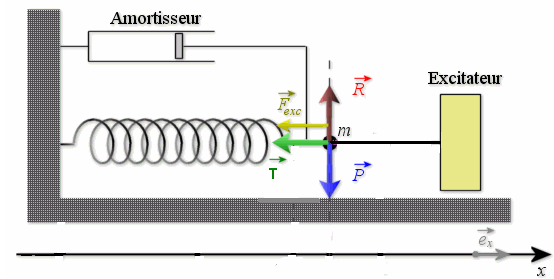
\includegraphics[width=0.8\linewidth]{img/amortisseur1.png}
\caption{Modèle d'un amortisseur}
\label{fig:image3}
\end{center}
\end{minipage}
\hfill
\begin{minipage}[c]{.40\linewidth}
\begin{center}
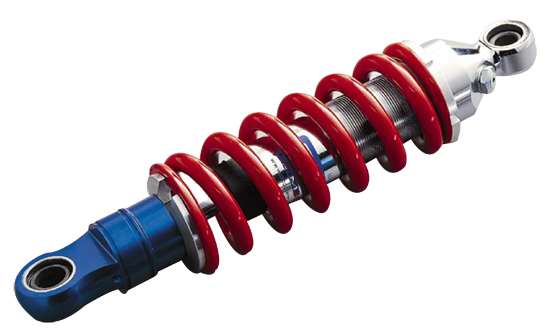
\includegraphics[width=0.8\linewidth]{img/amortisseur.jpg}
\caption{Amortisseur automobile}
\label{fig:image4}
\end{center}
La suspension d'un système est modélisée par un amortisseur et un ressort (figure \ref{fig:image4}). A t=0, un effort est exercé sur le système dont la masse est négligée.
\end{minipage}
\end{figure}

\paragraph{Question 1:}

Déterminer l'équation différentielle qui régit le système. L'entrée du système sera l'effort f(t) et la sortie l'oscillation de l'amortisseur. Les valeurs numériques sont les suivantes: $k=2.10^4N.m^{-1}$ et $\lambda=250N.s.m^{-1}$.

\paragraph{Question 2:}

Résoudre cette équation à l'aide des transformées de Laplace. Déterminer l'expression de la sortie s(t) quand l'entrée e(t) est un échelon de valeur $F=750N$ et en faire la représentation graphique pour $0<t<0,5s$.

\paragraph{Question 3:}

Déterminer $tr_{5\%}$, temps au bout duquel la sortie s(t) atteint 0,95 fois sa valeur à l'infini.

On présente à l'entrée une rampe d'effort $f(t)=\alpha.t.u(t)$ où u(t) est la fonction échelon avec $\alpha=100N.s^{-1}$. On rappelle que : u(t)=0 pour $t<0$ et u(t)=1 pour $t>0$.

Déterminer l'expression de la sortie s(t) et établir sur le même graphe les représentations graphiques de s(t) et e(t).

Déterminer l'écart de traînage $\epsilon_v=\lim\limits_{t \to +\infty}(e(t)-s(t))$ quand l'entrée e(t) est une rampe.

\begin{center}
\begin{tabular}{|c|c||c|c|}
\hline
Temporel $f(t)$ & Laplace $F(p)$ & 
Temporel $f(t)$ & Laplace $F(p)$ \\
\hline
\hline
 &&& \\
Dirac $\delta(t)$ &
$F(p)=1$ &
Échelon $ u(t)=k $&
$ U(p) = \frac{k}{p}$
\\
&&& \\
\hline
&&& \\
$f(t) = t^n\cdot u(t)$ &
$F(p)=\frac{n!}{p^{n+1}} $ &
$\forall t\in ]0,t_1 [ \quad f(t)= A$ & 
$F(p) =A \cdot \frac{1-e^{-pt_1}}{p} $\\
&&& \\
\hline
&&& \\
$f(t) = \sin \left( \omega_0 t\right) \cdot u(t)$ &
$F(p) = \frac{\omega_0}{p^2+\omega_0^2} $ &
$f(t) = \cos \left( \omega_0 t\right) \cdot u(t)$ & 
$F(p) = \frac{p}{p^2+\omega_0^2} $ \\
&&& \\
\hline
&&& \\
$f(t)= e^{-at}\cdot u(t)$ & 
$F(p)= \frac{1}{p+a}$ &
$f(t) = e^{-at}\sin\left( \omega_0 t\right) \cdot u(t)$ &
$F(p)=\frac{\omega_0}{\left( p+a\right)^2 + \omega_0^2}$  \\
&&& \\
\hline
&&& \\
$f(t) = e^{-at}\cos\left( \omega_0 t\right) \cdot u(t)$ &
$F(p)=\frac{p+a}{\left( p+a\right)^2 + \omega_0^2}$  &
$f(t)=t^ne^{-at}u(t)$ & $F(p)=\frac{n!}{\left( p+a\right)^{n+1}}$ \\
&&& \\
\hline
\end{tabular}
\end{center}

\newpage

\section{Réservoir}

%\subsection{Introduction}
%
%Définition de la transformation de Laplace :
%
%Soit f(t), une fonction de la variable temporelle réelle t et définie pour $t>0$. La transformée de Laplace de f(t), la fonction F(p), définie par l'intégrale généralisée :
%$F(p)=\int^{\infty}_0 e^{-pt}.f(t).dt$, notée $F(p)=L\left[f(t)\right]$
%
%p est la variable de Laplace, elle peut être une variable complexe ou réelle.
%
%\paragraph{Question 1:}
%
%Déterminer la transformée de Laplace de la fonction rampe.
%
%\paragraph{Question 2:}
%
%Déterminer la transformée de Laplace de la fonction $g(t)=\frac{1}{T}-\frac{1}{T}.e^{\frac{-t}{T}}$.
%
%\paragraph{Question 3:}
%
%Déterminer l'antécédent de la fonction $F(p)=\frac{p}{p.(1+Tp)}$ en décomposant F(p) en éléments simples. Tracer le graphe de l'original f(t) de F(p) pour $0<t<5T$.

\subsection{Présentation du système}

\begin{figure}[htbp]
\begin{minipage}[c]{.48\linewidth}
Un réservoir, est un aménagement accumulant l'eau de ruissellement d'un cours d'eau à l'aide d'un barrage. Dans le cas de notre étude seul trois paramètres nous intéressent, il s'agit de la hauteur de l'eau ($s(t)$, $s(0)=H_0$), le débit d'entrée ($e(t)$) et le débit de fuite ($q(t)$).
\end{minipage}
\hfill
\begin{minipage}[c]{.50\linewidth}
\begin{center}
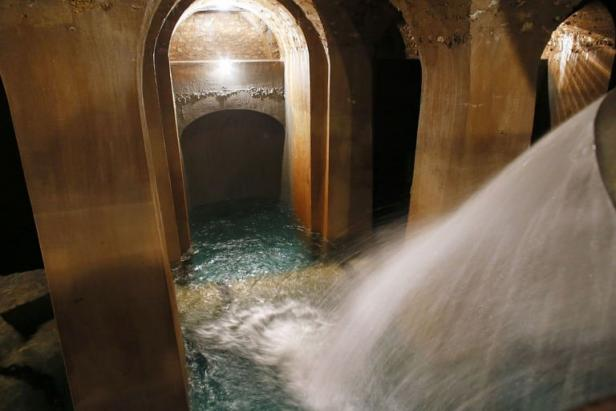
\includegraphics[width=0.8\linewidth]{img/reservoir.jpg}
\caption{Réservoir d'eau}
\label{fig:image5}
\end{center}
\end{minipage}
\end{figure}

\paragraph{Question 1:}

Déterminer l'équation différentielle qui régit le système. L'entrée du système sera le débit d'entrée e(t) et la sortie la hauteur de l'eau. Les valeurs numériques sont les suivantes: section du réservoir $S=100 m^2$ et $H_0=2m$. De plus, on fera l'hypothèse que le débit de la fuite sera proportionel au poid de l'eau dans le réservoir avec la relation suivante:$q(t)=K.P(t)$, avec $K=12.10^{-5}.m^3.N^{-1}.s^{-1}$.

\paragraph{Question 2:}

Résoudre cette équation à l'aide des transformées de Laplace. Déterminer l'expression de la sortie s(t) quand l'entrée e(t) est un échelon de valeur $F=750 m^3.s^{-1}$ et en faire la représentation graphique pour $0<t<5s$.

Le réservoir est-il en train de se remplir ou de se vider?

\paragraph{Question 3:}

Déterminer $tr_{5\%}$, temps au bout duquel la sortie s(t) atteint 0,95 fois sa valeur à l'infini.

On présente à l'entrée une rampe d'effort $f(t)=\alpha.t.u(t)$ où u(t) est la fonction échelon avec $\alpha=20 m^3.s^{-2}$. On rappelle que : u(t)=0 pour $t<0$ et u(t)=1 pour $t>0$.

Déterminer l'expression de la sortie s(t) et établir sur le même graphe les représentations graphiques de s(t) et e(t).

Déterminer l'écart de traînage $\epsilon_v=\lim\limits_{t \to +\infty}(e(t)-s(t))$ quand l'entrée e(t) est une rampe.

\begin{center}
\begin{tabular}{|c|c||c|c|}
\hline
Temporel $f(t)$ & Laplace $F(p)$ & 
Temporel $f(t)$ & Laplace $F(p)$ \\
\hline
\hline
 &&& \\
Dirac $\delta(t)$ &
$F(p)=1$ &
Échelon $ u(t)=k $&
$ U(p) = \frac{k}{p}$
\\
&&& \\
\hline
&&& \\
$f(t) = t^n\cdot u(t)$ &
$F(p)=\frac{n!}{p^{n+1}} $ &
$\forall t\in ]0,t_1 [ \quad f(t)= A$ & 
$F(p) =A \cdot \frac{1-e^{-pt_1}}{p} $\\
&&& \\
\hline
&&& \\
$f(t) = \sin \left( \omega_0 t\right) \cdot u(t)$ &
$F(p) = \frac{\omega_0}{p^2+\omega_0^2} $ &
$f(t) = \cos \left( \omega_0 t\right) \cdot u(t)$ & 
$F(p) = \frac{p}{p^2+\omega_0^2} $ \\
&&& \\
\hline
&&& \\
$f(t)= e^{-at}\cdot u(t)$ & 
$F(p)= \frac{1}{p+a}$ &
$f(t) = e^{-at}\sin\left( \omega_0 t\right) \cdot u(t)$ &
$F(p)=\frac{\omega_0}{\left( p+a\right)^2 + \omega_0^2}$  \\
&&& \\
\hline
&&& \\
$f(t) = e^{-at}\cos\left( \omega_0 t\right) \cdot u(t)$ &
$F(p)=\frac{p+a}{\left( p+a\right)^2 + \omega_0^2}$  &
$f(t)=t^ne^{-at}u(t)$ & $F(p)=\frac{n!}{\left( p+a\right)^{n+1}}$ \\
&&& \\
\hline
\end{tabular}
\end{center}

\newpage

\section{Amortisseur du second ordre}

Cette étude s'intéresse au mouvement d'une roue par rapport au châssis par l'intermédiaire d'un amortisseur et ressort. Ce système peut être modélisé par une masse reliée en série à un ressort et un amortisseur montés en parallèle. 

\begin{figure}[htbp]
\begin{minipage}[c]{.48\linewidth}
\begin{center}
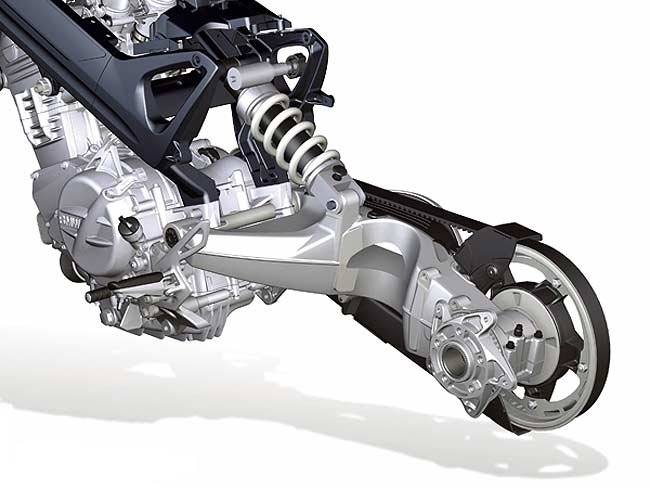
\includegraphics[width=0.8\linewidth]{img/moto.jpg}
\caption{Amortisseur moto}
\label{fig:image6}
\end{center}
\end{minipage}
\hfill
\begin{minipage}[c]{.50\linewidth}
\begin{center}
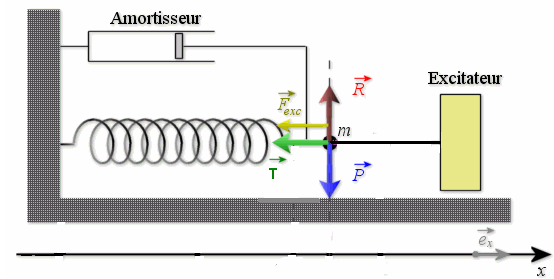
\includegraphics[width=0.8\linewidth]{img/amortisseur1.png}
\caption{Schéma de l'amortisseur}
\label{fig:image7}
\end{center}
\end{minipage}
\end{figure}

 
On note e(t) la force exercée sur la masse $M$ et $x(t)$ la position de cette masse par rapport à l'équilibre. La masse $M$ est soumise :  
\begin{itemize}
 \item à l'action $e(t)$
 \item à l'action du ressort : $-k.x(t)$
 \item à l'action de l'amortisseur hydraulique : $-f.v(t)$
\end{itemize}

En appliquant le principe fondamental de la dynamique sur la masse M, on obtient l'équation :
$m.a(t)=e(t)-k.x(t)-f.v(t)$

\paragraph{Question 1 :} Donner la transformée de Laplace de cette équation. 
\paragraph{Question 2 :} Donner la fonction de transfert du système $H(p)=\frac{X(p)}{E(p)}$, en identifiez la classe, l'ordre et le gain. 
\paragraph{Question 3 :} Calculer les paramètres, $K$, $\omega_m$ et $z$. Tracer la réponse à un échelon $(L(u(t))=\frac{1}{p})$. 
\paragraph{Question 4 :} Calculer la réponse temporelle à cet échelon pour $\xi=3$, $K=12$ et $\omega_0=200rad.s^{-1}$.

\begin{center}
\begin{tabular}{|c|c||c|c|}
\hline
Temporel $f(t)$ & Laplace $F(p)$ & 
Temporel $f(t)$ & Laplace $F(p)$ \\
\hline
\hline
 &&& \\
Dirac $\delta(t)$ &
$F(p)=1$ &
Échelon $ u(t)=k $&
$ U(p) = \frac{k}{p}$
\\
&&& \\
\hline
&&& \\
$f(t) = t^n\cdot u(t)$ &
$F(p)=\frac{n!}{p^{n+1}} $ &
$\forall t\in ]0,t_1 [ \quad f(t)= A$ & 
$F(p) =A \cdot \frac{1-e^{-pt_1}}{p} $\\
&&& \\
\hline
&&& \\
$f(t) = \sin \left( \omega_0 t\right) \cdot u(t)$ &
$F(p) = \frac{\omega_0}{p^2+\omega_0^2} $ &
$f(t) = \cos \left( \omega_0 t\right) \cdot u(t)$ & 
$F(p) = \frac{p}{p^2+\omega_0^2} $ \\
&&& \\
\hline
&&& \\
$f(t)= e^{-at}\cdot u(t)$ & 
$F(p)= \frac{1}{p+a}$ &
$f(t) = e^{-at}\sin\left( \omega_0 t\right) \cdot u(t)$ &
$F(p)=\frac{\omega_0}{\left( p+a\right)^2 + \omega_0^2}$  \\
&&& \\
\hline
&&& \\
$f(t) = e^{-at}\cos\left( \omega_0 t\right) \cdot u(t)$ &
$F(p)=\frac{p+a}{\left( p+a\right)^2 + \omega_0^2}$  &
$f(t)=t^ne^{-at}u(t)$ & $F(p)=\frac{n!}{\left( p+a\right)^{n+1}}$ \\
&&& \\
\hline
\end{tabular}
\end{center}

\newpage

\section{Moteur électrique à courant continu}

La rotation des bobines dans le champ magnétique produit une force électromotrice $e(t)$ proportionnelle à la vitesse de rotation du rotor par rapport au bâti : $\omega(t)$.

$e(t)=K_e.w(t)$ où $K_e$ est la constante électrique du moteur.

L'intensité électrique $i(t)$ qui traverse les bobines de l'induit produit un couple moteur sur l'arbre du rotor noté $Cm(t)$ proportionnel à cette intensité $i(t)$ : $Cm(t)=K_t.i(t)$ où $K_t$ est la constante de 
couple du moteur. 

\begin{figure}[htbp]
\begin{minipage}[c]{.48\linewidth}
\begin{center}
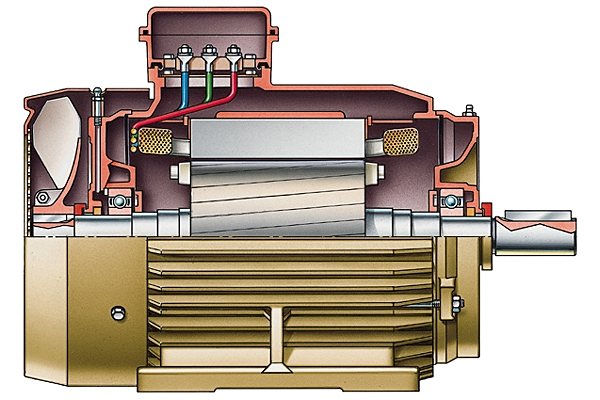
\includegraphics[width=0.8\linewidth]{img/moteur.jpg}
\caption{Moteur électrique}
\label{fig:image8}
\end{center}
\end{minipage}
\hfill
\begin{minipage}[c]{.50\linewidth}
\begin{center}
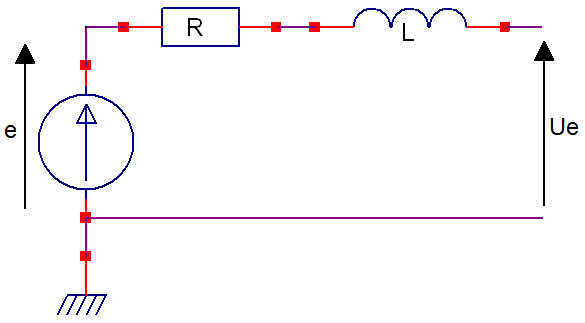
\includegraphics[width=0.8\linewidth]{img/moteur_s.png}
\caption{Modèle électrique du moteur}
\label{fig:image9}
\end{center}
\end{minipage}
\end{figure}

L'arbre moteur est soumis à un couple de frottement visqueux proportionnel à la vitesse de rotation du rotor par rapport au bâti. Le moment d'inertie équivalent de l'ensemble des masses en mouvement dans la chaîne cinématique est noté $J$. Le principe fondamental de la dynamique donne alors : $Cm(t)=f.w(t)+J.\dot{w}(t)$.

 
\paragraph{Question 1 :} Ecrivez les relations entre les tensions aux bornes de la résistance R et de l'inductance L. En déduire l'équation différentielle qui régit le circuit électrique par application des lois de Kirchoff.

\paragraph{Question 2 :} Donner les transformées de Laplace de ces équations. 

\paragraph{Question 3 :} Donner la fonction de transfert du système $H(p)=\frac{\Omega(p)}{U(p)}$, en identifiez la classe, l'ordre et le gain.

\paragraph{Question 4 :} Calculer les paramètres, $K$, $\omega_m$ et $z$. Tracer la réponse à un échelon $(L(u(t))=\frac{1}{p})$.

\paragraph{Question 5 :} Calculer la réponse temporelle à cet échelon pour $\xi=2$, $K=18$ et $\omega_0=230rad.s^{-1}$.

\begin{center}
\begin{tabular}{|c|c||c|c|}
\hline
Temporel $f(t)$ & Laplace $F(p)$ & 
Temporel $f(t)$ & Laplace $F(p)$ \\
\hline
\hline
 &&& \\
Dirac $\delta(t)$ &
$F(p)=1$ &
Échelon $ u(t)=k $&
$ U(p) = \frac{k}{p}$
\\
&&& \\
\hline
&&& \\
$f(t) = t^n\cdot u(t)$ &
$F(p)=\frac{n!}{p^{n+1}} $ &
$\forall t\in ]0,t_1 [ \quad f(t)= A$ & 
$F(p) =A \cdot \frac{1-e^{-pt_1}}{p} $\\
&&& \\
\hline
&&& \\
$f(t) = \sin \left( \omega_0 t\right) \cdot u(t)$ &
$F(p) = \frac{\omega_0}{p^2+\omega_0^2} $ &
$f(t) = \cos \left( \omega_0 t\right) \cdot u(t)$ & 
$F(p) = \frac{p}{p^2+\omega_0^2} $ \\
&&& \\
\hline
&&& \\
$f(t)= e^{-at}\cdot u(t)$ & 
$F(p)= \frac{1}{p+a}$ &
$f(t) = e^{-at}\sin\left( \omega_0 t\right) \cdot u(t)$ &
$F(p)=\frac{\omega_0}{\left( p+a\right)^2 + \omega_0^2}$  \\
&&& \\
\hline
&&& \\
$f(t) = e^{-at}\cos\left( \omega_0 t\right) \cdot u(t)$ &
$F(p)=\frac{p+a}{\left( p+a\right)^2 + \omega_0^2}$  &
$f(t)=t^ne^{-at}u(t)$ & $F(p)=\frac{n!}{\left( p+a\right)^{n+1}}$ \\
&&& \\
\hline
\end{tabular}
\end{center}

\newpage

\section{Vérin piloté}

Ce vérin permet de guider un bateau automatiquement.

Le comportement du vérin peut alors être modélisé à partir du modèle de structure ci-dessous et du paramétrage qui lui est associé.

\begin{figure}[htbp]
\begin{minipage}[c]{.48\linewidth}
\begin{center}
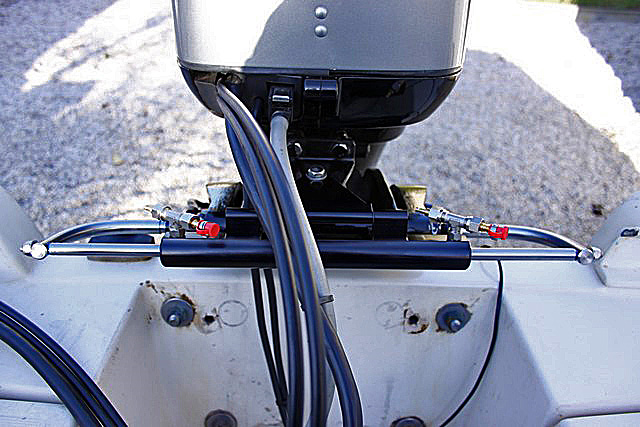
\includegraphics[width=0.8\linewidth]{img/verin.png}
\caption{Vérin installé}
\label{fig:image10}
\end{center}
\end{minipage}
\hfill
\begin{minipage}[c]{.50\linewidth}
\begin{center}
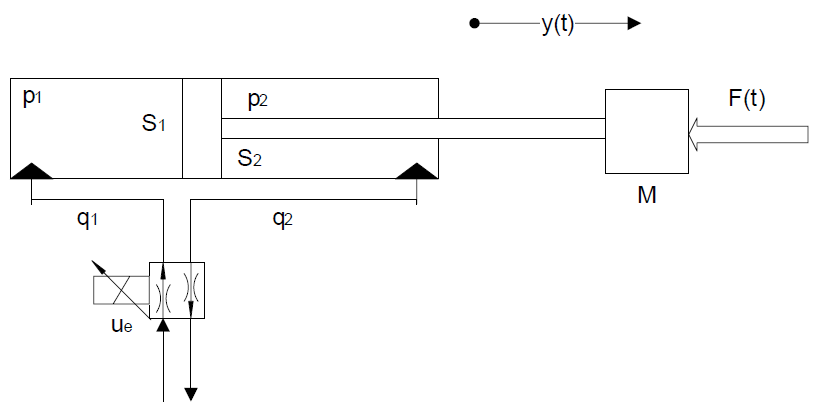
\includegraphics[width=\linewidth]{img/verin2.png}
\caption{Modèle du vérin}
\label{fig:image11}
\end{center}
\end{minipage}
\end{figure}

\begin{itemize}
 \item $M = 10^4 kg$ : masse de l'équipage mobile,
 \item $f = 3.10^6 N.m^{-1}.s$ : résistance due aux frottements visqueux,
 \item $K = 2,5.10^7 N.m^{-1}$ : la raideur hydraulique du vérin, 
 \item $S_1 = 5.10^{-2} m^2$ : la surface du piston de la chambre d'admission.
\end{itemize}

L'ensemble \og équipage mobile \fg est formé par : le tiroir, l'effort variable dû à la ferraille, noté $F(t)$ et la tige du piston du vérin. La position notée $y(t)$ est fonction du débit d'huile, noté $q_1(t)$, à l'entrée de la chambre d'admission du vérin. On se place dans l'hypothèse de petit déplacement autour d'un point de fonctionnement (position particulière d'équilibre). Le système peut donc être considéré comme linéaire, continu et invariant.

Modélisation de l'équipage mobile. L'équation temporelle donnant le déplacement $y_1(t)$ en fonction du débit $q_1(t)$ pour un effort $F(t)$ nul est telle que :

$M.\frac{d^2y_1(t)}{dt^2}=K.\int_0^t \frac{q_1(\tau)}{S_1}.d\tau-K.y_1(t)-f\frac{d y_1(t)}{dt}$.

L'équation temporelle donnant le déplacement $y_2(t)$ en fonction de l'effort $F(t)$ pour un débit $q_1(t)$ nul est telle que :

$M.\frac{d^2y_2(t)}{dt^2}=-K.y_2(t)-f\frac{d y_2(t)}{dt}+F(t)$.

\paragraph{Question 1 :} En supposant que les conditions initiales sont nulles, donner dans le domaine de Laplace et sous forme canonique : 

\begin{itemize}
 \item La fonction de transfert : $H_1(p)=\frac{Y_1(p)}{Q_1(p)}$ liant le déplacement $y_1(t)$ au débit $q_1(t)$ pour un effort $F(t)$ nul, 
 \item La fonction de transfert : $H_2(p)=\frac{Y_2(p)}{F(p)}$ liant le déplacement $y_2(t)$ à l'effort $F(t)$ pour un débit $q_1(t)$ nul.
\end{itemize}
 
En donner l'ordre et la classe.

\paragraph{Question 2 :} En appliquant le principe de superposition, donner l'équation, dans le domaine de Laplace, liant le déplacement $Y(p)$ au débit $Q_1(p)$ et à l'effort $F(p)$.

Modélisation générale du fonctionnement de l'ensemble vérin et distribution. 

Pour étudier l'influence du débit, on néglige la contribution de l'effort $F(t)$. La fonction de transfert déplacement-débit est alors :

$G(p)=\frac{Y(p)}{Q_1(p)}=\frac{1}{p.S_1.(1+\frac{1}{K}.(f.p+M.p^2))}$

On admettra que ce résultat est généralisable pour toute position de la tige de vérin. Un servodistributeur proportionnel délivre un débit d'huile $q_1(t)$ proportionnel à sa tension de commande $u_e(t)$ tel que : $q_1(t)= Ke.u_e(t)$, avec $Ke=2.10^{-4} m^3.s^{-1}.V^{-1}$. Un détecteur de position délivre une tension $u_s(t)$ proportionnelle à la position $y(t)$ du tiroir telle que : $u_s(t)=Kc.y(t)$, avec $Kc= 10^3 V.m^{-1}$. 

\paragraph{Question 3 :} En déduire la fonction de transfert suivante: $\frac{U_s(p)}{U_e(p)}$.

\paragraph{Question 4 :} Calculer $u_s(t)$ pour une entrée en échelon unitaire.

\begin{center}
\begin{tabular}{|c|c||c|c|}
\hline
Temporel $f(t)$ & Laplace $F(p)$ & 
Temporel $f(t)$ & Laplace $F(p)$ \\
\hline
\hline
 &&& \\
Dirac $\delta(t)$ &
$F(p)=1$ &
Échelon $ u(t)=k $&
$ U(p) = \frac{k}{p}$
\\
&&& \\
\hline
&&& \\
$f(t) = t^n\cdot u(t)$ &
$F(p)=\frac{n!}{p^{n+1}} $ &
$\forall t\in ]0,t_1 [ \quad f(t)= A$ & 
$F(p) =A \cdot \frac{1-e^{-pt_1}}{p} $\\
&&& \\
\hline
&&& \\
$f(t) = \sin \left( \omega_0 t\right) \cdot u(t)$ &
$F(p) = \frac{\omega_0}{p^2+\omega_0^2} $ &
$f(t) = \cos \left( \omega_0 t\right) \cdot u(t)$ & 
$F(p) = \frac{p}{p^2+\omega_0^2} $ \\
&&& \\
\hline
&&& \\
$f(t)= e^{-at}\cdot u(t)$ & 
$F(p)= \frac{1}{p+a}$ &
$f(t) = e^{-at}\sin\left( \omega_0 t\right) \cdot u(t)$ &
$F(p)=\frac{\omega_0}{\left( p+a\right)^2 + \omega_0^2}$  \\
&&& \\
\hline
&&& \\
$f(t) = e^{-at}\cos\left( \omega_0 t\right) \cdot u(t)$ &
$F(p)=\frac{p+a}{\left( p+a\right)^2 + \omega_0^2}$  &
$f(t)=t^ne^{-at}u(t)$ & $F(p)=\frac{n!}{\left( p+a\right)^{n+1}}$ \\
&&& \\
\hline
\end{tabular}
\end{center}

\newpage

\section{Chaudière}

L'étude porte sur la montée en température de l'eau qui sert à chauffer les pièces au travers de radiateurs. Cette température est obtenue à partir d'une puissance calorifique fournie par le bois brûlé au niveau du foyer réfractaire de la chaudière.

\begin{figure}[htbp]
\begin{minipage}[c]{.48\linewidth}	
\begin{center}
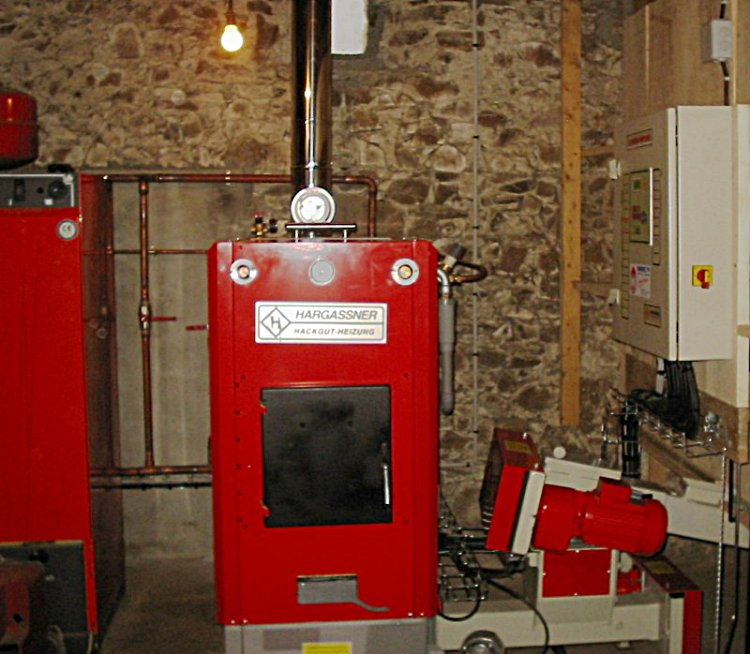
\includegraphics[width=0.7\linewidth]{img/chaudiere.png}
\caption{Chaudière}
\label{fig:image12}
\end{center}
\end{minipage}
\hfill
\begin{minipage}[c]{.50\linewidth}
\begin{center}
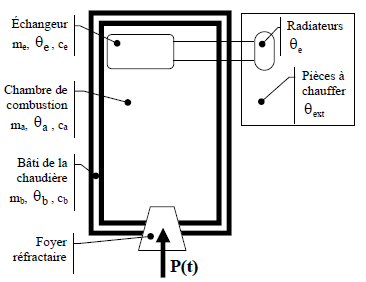
\includegraphics[width=0.8\linewidth]{img/chaudiere2.png}
\caption{Schéma de la chaudière}
\label{fig:image13}
\end{center}
\end{minipage}
\end{figure}

p(t) est la puissance calorifique en Watt fournie par le bois brulé. L'air situé dans la chambre de combustion permet de monter à la température $\theta_e(t)$ l'eau située dans l'échangeur. L'eau chaude, au travers des radiateurs permet de chauffer les pièces à une température $\theta_{ext}(t)$.

On note :
\begin{itemize}
 \item $\theta_b(t)$ la température du bâti de la chaudière,
 \item $m_b$ la masse du bâti à monter en température, $m_b=200kg$,
 \item $c_b$ la capacité calorifique massique du bâti, $c_b=500J.kg^{-1}.K^{-1}$,
 \item $\theta_a(t)$ la température de l'air dans la chambre de combustion,
 \item $m_a$ la masse de l'air à monter en température ; $m_a=2kg$,
 \item $c_a$ la capacité calorifique massique de l'air, $c_a=700J.kg^{-1}.K^{-1}$,
 \item $\theta_e(t)$ la température de l'eau dans l'échangeur et les radiateurs,
 \item $m_e$ la masse de l'eau à monter en température dans l'échangeur, $m_e=50kg$,
 \item $c_e$ la capacité calorifique massique de l'eau, $c_e=4000J.kg^{-1}.K^{-1}$,
 \item $\theta_{ext}(t)$ la température ambiante des pièces à chauffer.
\end{itemize}

D'après le principe de conservation:

$m_b.c_b.\frac{d\theta_b(t)}{dt}+K_{ab}.(\theta_b(t)-\theta_a(t))=p(t)$

$m_a.c_a.\frac{d\theta_a(t)}{dt}+K_{ae}.(\theta_a(t)-\theta_e(t))=K_{ab}.(\theta_b(t)-\theta_a(t))$

$m_e.c_e.\frac{d\theta_e(t)}{dt}+K_{ae}.(\theta_e(t)-\theta_{ext}(t))=K_{ae}.(\theta_a(t)-\theta_e(t))$

Avec :
\begin{itemize}
 \item $K_{ab}$ la conductance thermique bâti/air dans la chambre de combustion, $K_{ab}=40 J.s^{-1}.K^{-1}$,
 \item $K_{ae}$ la conductance thermique air/eau au travers de l'échangeur/radiateurs. $K_{ae}=400 J.s^{-1}.K^{-1}$.
\end{itemize}

On suppose que le corps de chauffe est parfaitement isolé de l'extérieur.

Les transformées de Laplace seront notées : $L[\theta_i(t)]=T_i(p)$ et $L[p(t)]=P(p)$.

\paragraph{Question 1 :} En supposant que les conditions initiales sont nulles (conditions de Heaviside), donner dans le domaine de Laplace, la transformée des équations différentielles précédentes.

\paragraph{Question 2 :} Exprimer $T_b(p)$ en fonction de $T_a(p)$ et de $P(p)$ en faisant apparaitre les variables $m_b$, $c_b$ et $K_{ab}$ mettre sous la forme : $T_b(p)=H_1(p).T_a(p)+H_2(p).P(p)$.

Préciser l'ordre du système définit par la fonction de transfert $H_1(p)$, ainsi que, littéralement, ses caractéristiques.
Calculer la valeur numérique approchée de $\tau_1$, la constante de temps de ce système.

\paragraph{Question 3 :} Exprimer $T_a(p)$ en fonction de $T_e(p)$ et de $T_b(p)$ en faisant apparaitre les variables $m_a$, $c_a$, $K_{ae}$ et $K_{ab}$.

Mettre $T_a(p)$ sous la forme $T_a(p)=H_3(p).T_e(p)+H_4(p).T_b(p)$.

Préciser l'ordre des systèmes définis par les fonctions de transfert respectives $H_3(p)$ et $H_4(p)$, ainsi que, littéralement, leurs caractéristiques.

Calculer la valeur numérique approchée de $\tau_3$, la constante de temps de ces systèmes.

\begin{center}
\begin{tabular}{|c|c||c|c|}
\hline
Temporel $f(t)$ & Laplace $F(p)$ & 
Temporel $f(t)$ & Laplace $F(p)$ \\
\hline
\hline
 &&& \\
Dirac $\delta(t)$ &
$F(p)=1$ &
Échelon $ u(t)=k $&
$ U(p) = \frac{k}{p}$
\\
&&& \\
\hline
&&& \\
$f(t) = t^n\cdot u(t)$ &
$F(p)=\frac{n!}{p^{n+1}} $ &
$\forall t\in ]0,t_1 [ \quad f(t)= A$ & 
$F(p) =A \cdot \frac{1-e^{-pt_1}}{p} $\\
&&& \\
\hline
&&& \\
$f(t) = \sin \left( \omega_0 t\right) \cdot u(t)$ &
$F(p) = \frac{\omega_0}{p^2+\omega_0^2} $ &
$f(t) = \cos \left( \omega_0 t\right) \cdot u(t)$ & 
$F(p) = \frac{p}{p^2+\omega_0^2} $ \\
&&& \\
\hline
&&& \\
$f(t)= e^{-at}\cdot u(t)$ & 
$F(p)= \frac{1}{p+a}$ &
$f(t) = e^{-at}\sin\left( \omega_0 t\right) \cdot u(t)$ &
$F(p)=\frac{\omega_0}{\left( p+a\right)^2 + \omega_0^2}$  \\
&&& \\
\hline
&&& \\
$f(t) = e^{-at}\cos\left( \omega_0 t\right) \cdot u(t)$ &
$F(p)=\frac{p+a}{\left( p+a\right)^2 + \omega_0^2}$  &
$f(t)=t^ne^{-at}u(t)$ & $F(p)=\frac{n!}{\left( p+a\right)^{n+1}}$ \\
&&& \\
\hline
\end{tabular}
\end{center}

\newpage

\section{Identification fréquentielle 1}

L'analyse fréquentielle d'un système a donné le tracé suivant.

\begin{center}
 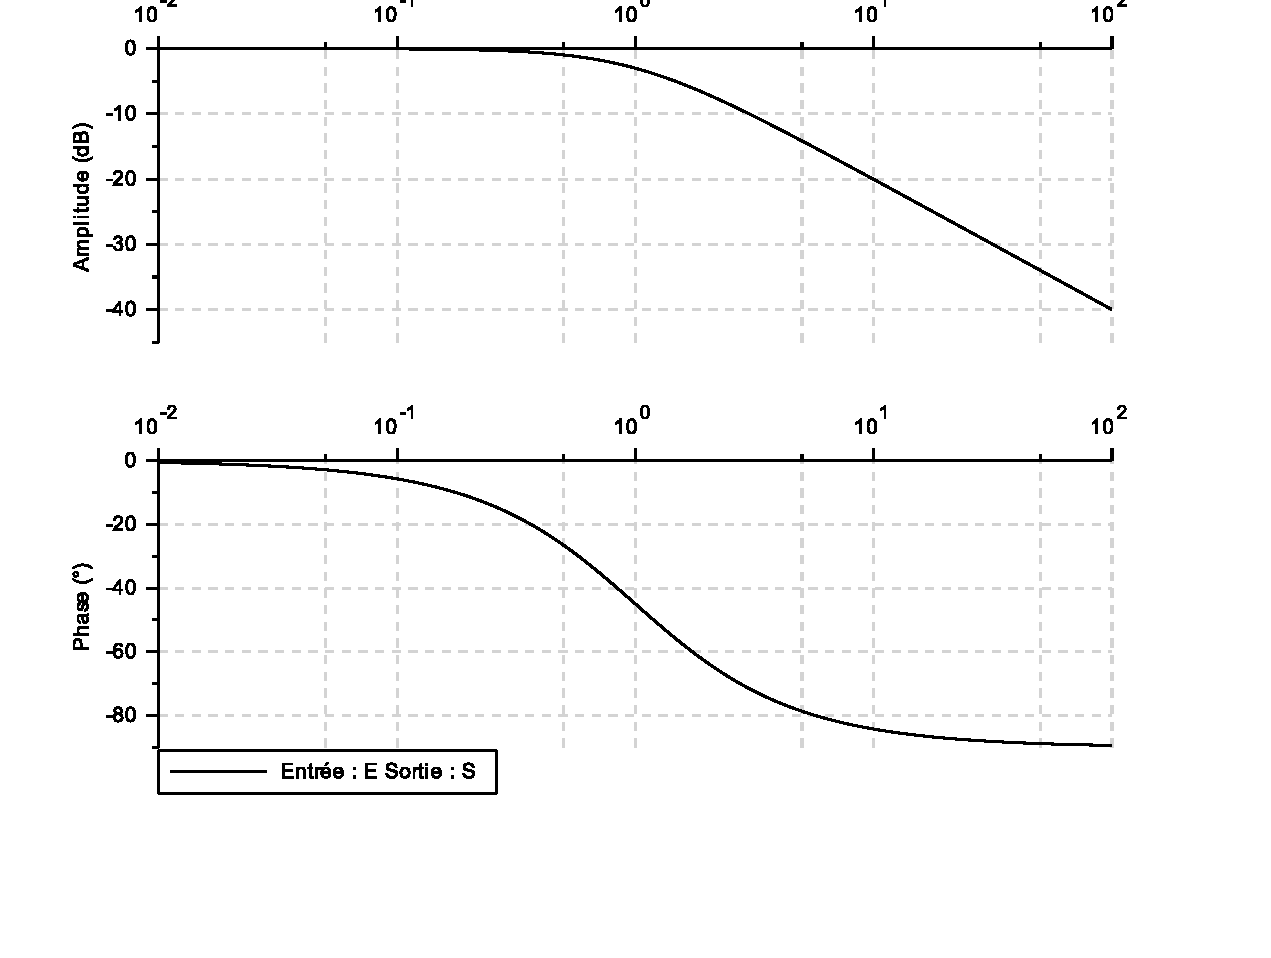
\includegraphics[width=0.8\linewidth]{img/Bode1}
\end{center} 

\paragraph{Question 1:} Tracer les asymptotes à cette courbe.

\paragraph{Question 2:} Déterminer la fonction de transfert correspondante.

\newpage ~\ \newpage

\section{Identification fréquentielle 2}

L'analyse fréquentielle d'un système a donné le tracé suivant.

\begin{center}
 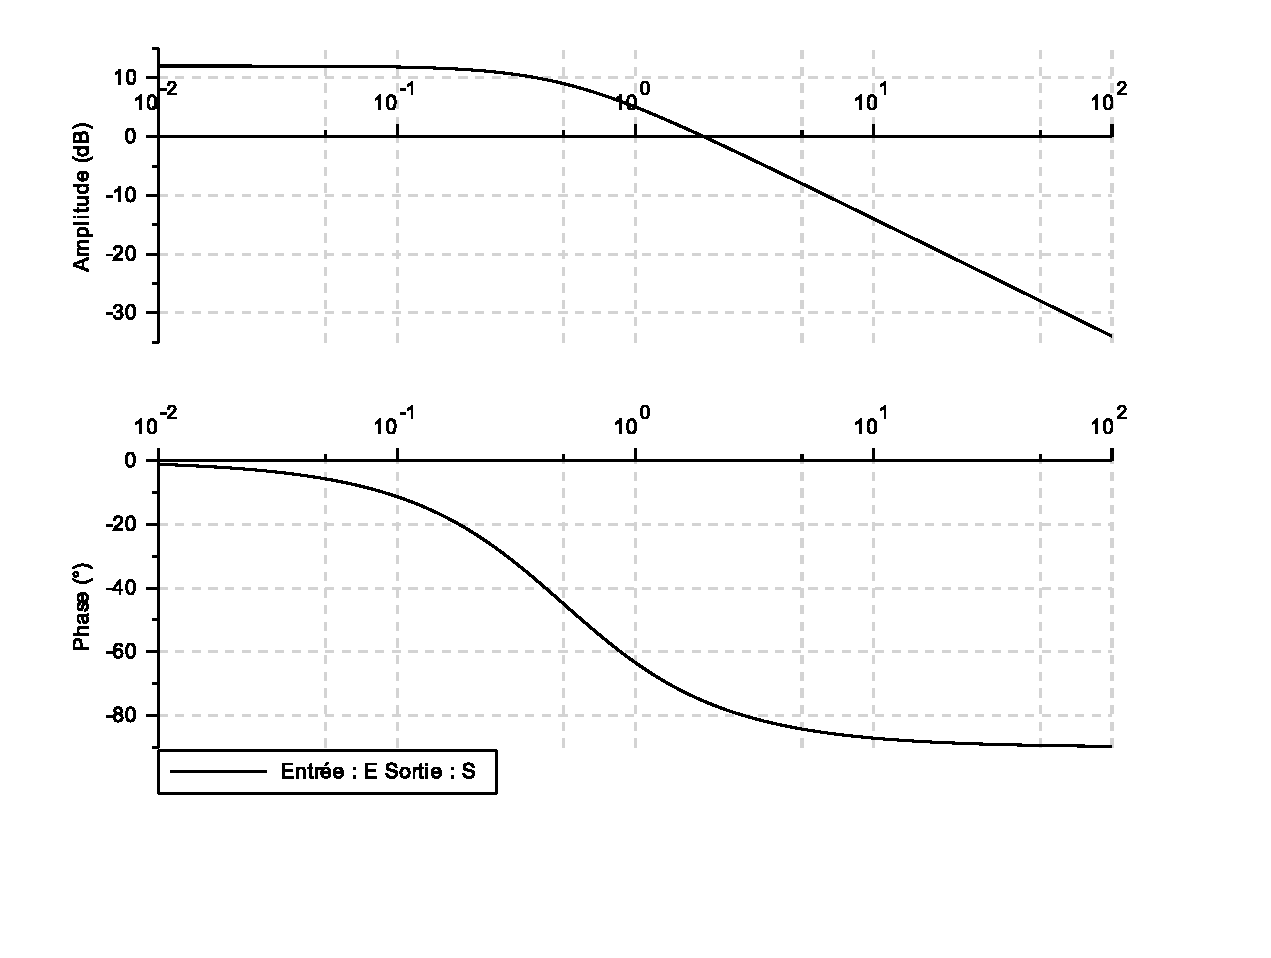
\includegraphics[width=0.8\linewidth]{img/Bode2}
\end{center} 

\paragraph{Question 1:} Tracer les asymptotes à cette courbe.

\paragraph{Question 2:} Déterminer la fonction de transfert correspondante.

\newpage ~\ \newpage

\section{Identification fréquentielle 3}

L'analyse fréquentielle d'un système a donné le tracé suivant.

\begin{center}
 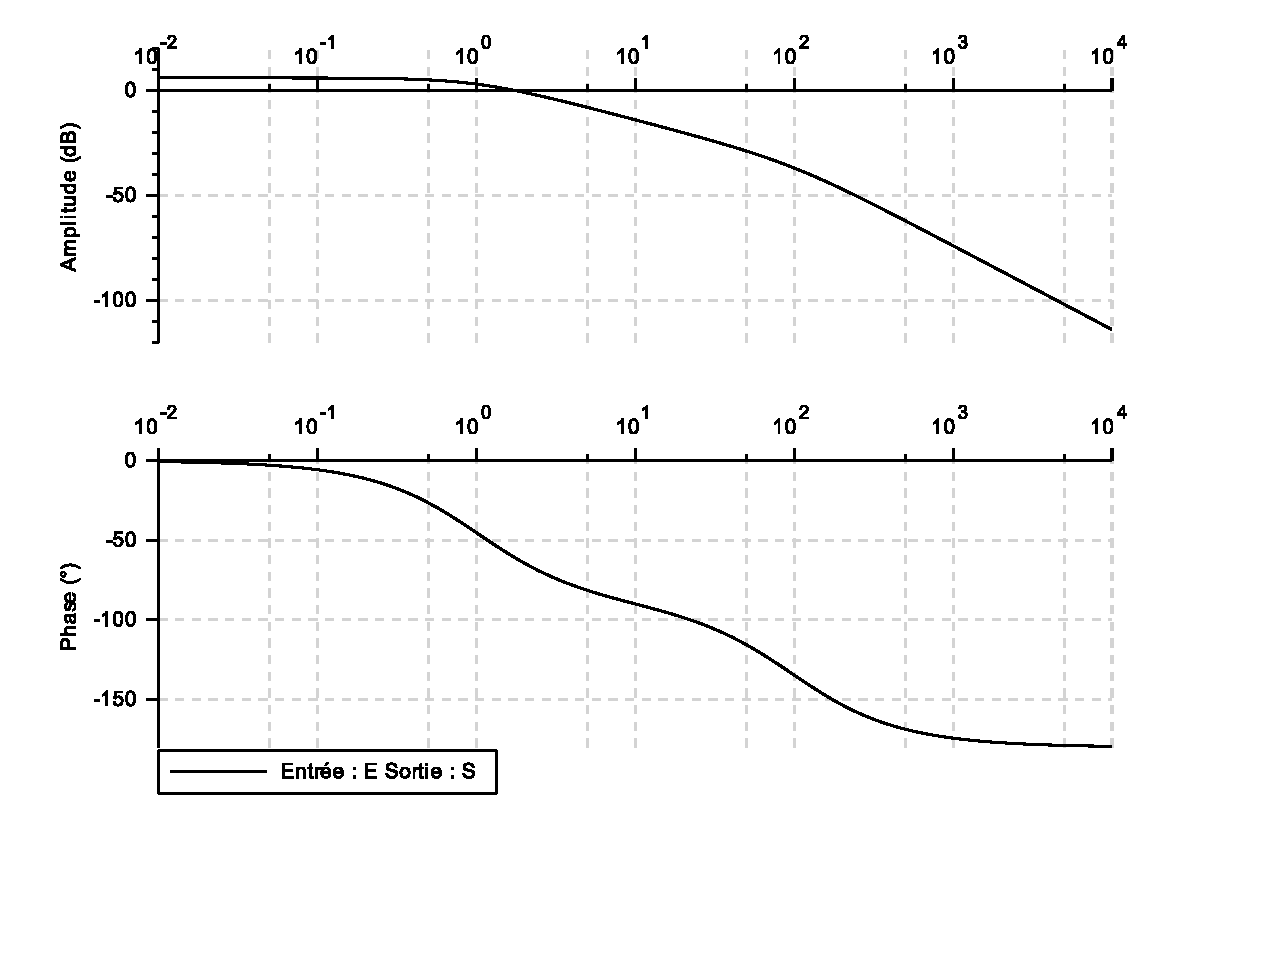
\includegraphics[width=0.8\linewidth]{img/Bode4}
\end{center} 

\paragraph{Question 1:} Tracer les asymptotes à cette courbe.

\paragraph{Question 2:} Déterminer la fonction de transfert correspondante.

\newpage ~\ \newpage

\section{Identification fréquentielle 4}

L'analyse fréquentielle d'un système a donné le tracé suivant.

\begin{center}
 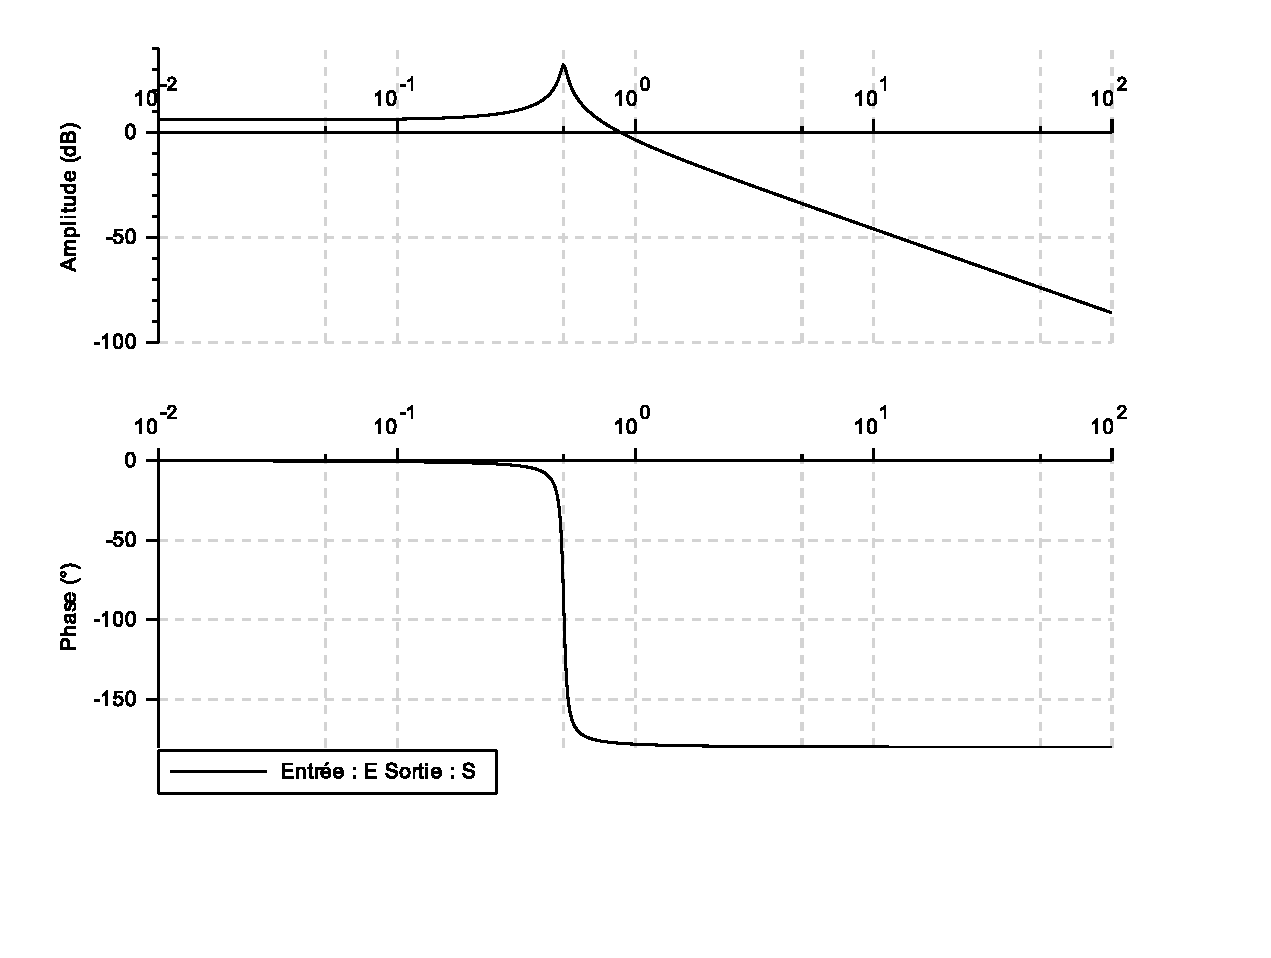
\includegraphics[width=0.8\linewidth]{img/Bode3}
\end{center} 

\paragraph{Question 1:} Tracer les asymptotes à cette courbe.

\paragraph{Question 2:} Déterminer la fonction de transfert correspondante.

\end{document}

\newpage

\pagestyle{correction}\setcounter{section}{0}

\section{Identification fréquentielle 1}

L'analyse fréquentielle d'un système a donné le tracé suivant.


\paragraph{Question 1:} Tracer les asymptotes à cette courbe.

\begin{center}
 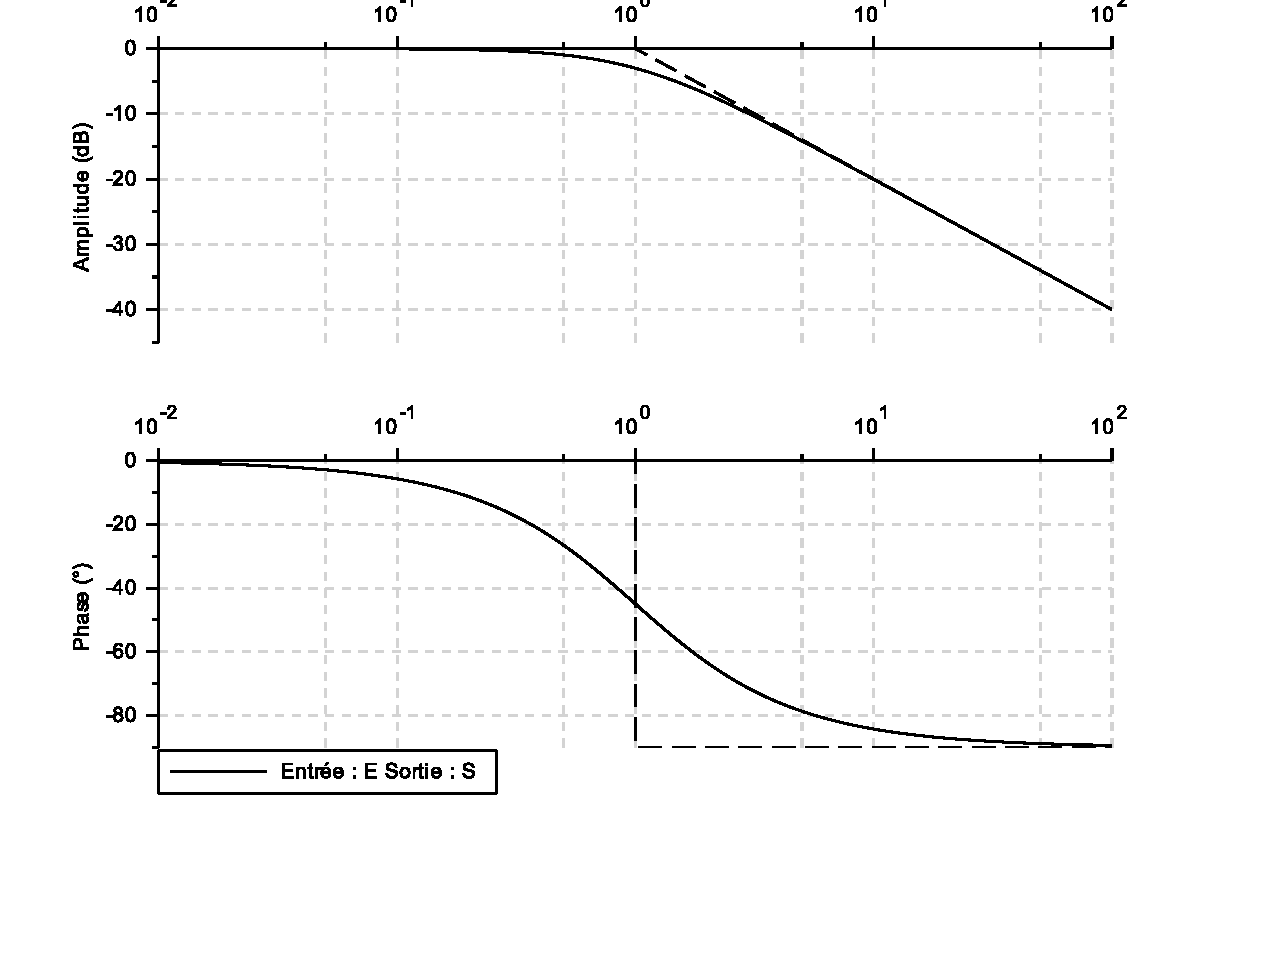
\includegraphics[width=0.8\linewidth]{img/Bode1_c}
\end{center} 

\paragraph{Question 2:} Déterminer la fonction de transfert correspondante.

La tangente à l'infini est de $-20dB/dec$, il s'agit donc d'un premier ordre.

La tangente au départ vaut $0$, donc $20*log(K)=0$, donc $K=10^0=1$.

La pulsation de coupure est $w_0=10^0$, donc $\tau=\dfrac{1}{1}=1$.

La fonction de transfert est donc $H(p)=\dfrac{1}{1+p}$.

\newpage

\section{Identification fréquentielle 2}

L'analyse fréquentielle d'un système a donné le tracé suivant.

\paragraph{Question 1:} Tracer les asymptotes à cette courbe.

\begin{center}
 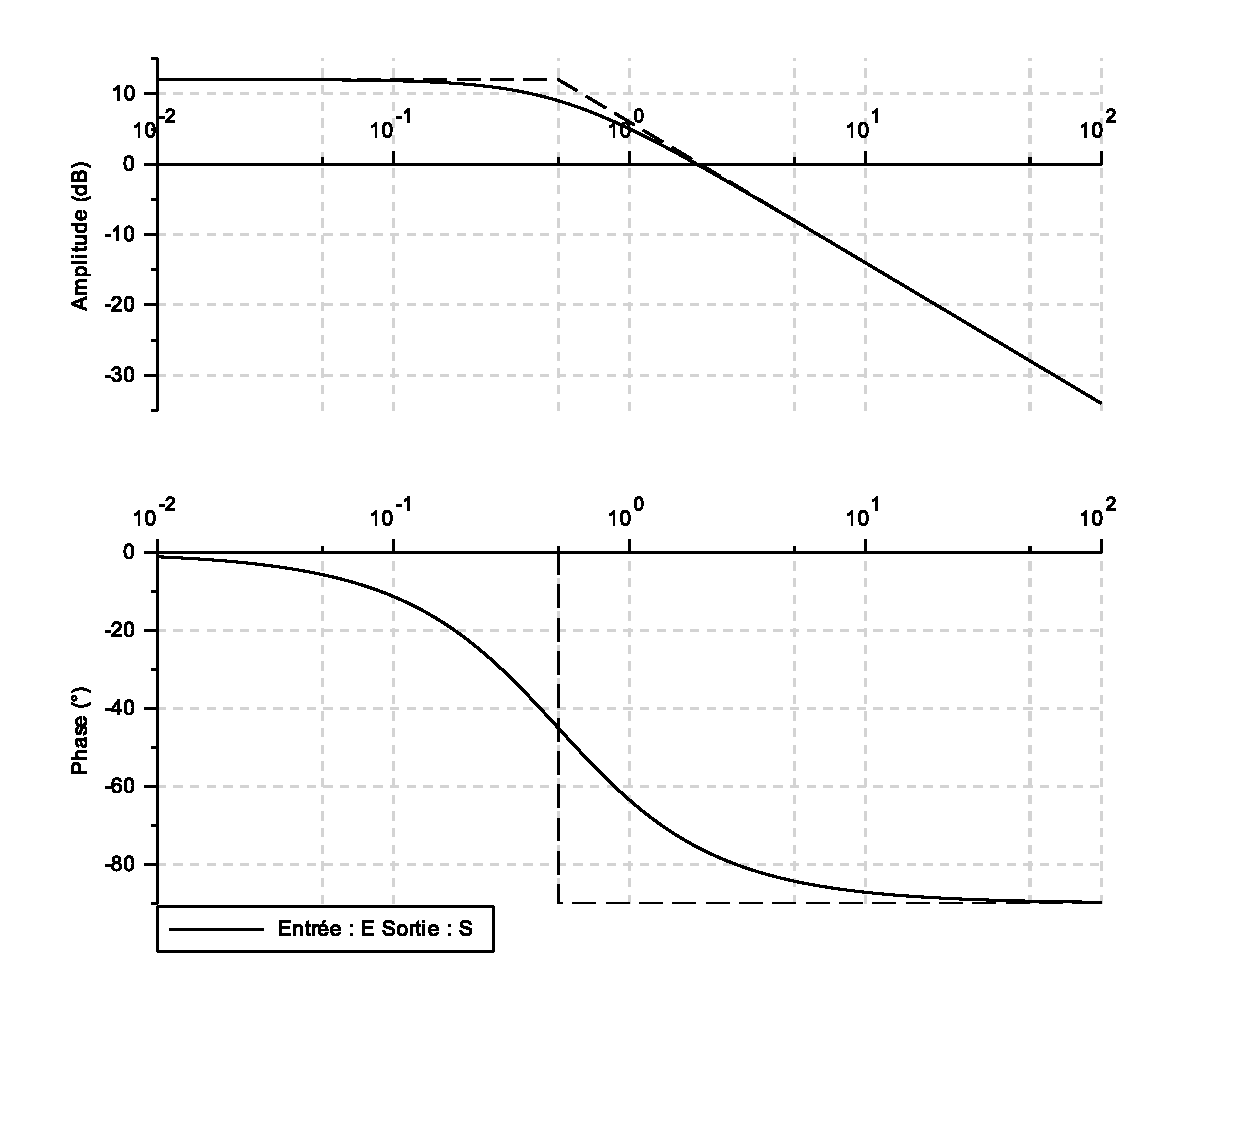
\includegraphics[width=0.8\linewidth]{img/Bode2_c}
\end{center} 
\paragraph{Question 2:} Déterminer la fonction de transfert correspondante.

La tangente à l'infini est de $-20dB/dec$, il s'agit donc d'un premier ordre.

La tangente au départ vaut environ $12$, donc $20*log(K)=12$, donc $K\simeq 4$.

La pulsation de coupure est $w_0\simeq 0.5$, donc $\tau\simeq 2$.

La fonction de transfert est donc $H(p)=\dfrac{4}{1+2*p}$.

\newpage

\section{Identification fréquentielle 4}

L'analyse fréquentielle d'un système a donné le tracé suivant.

\paragraph{Question 1:} Tracer les asymptotes à cette courbe.

\begin{center}
 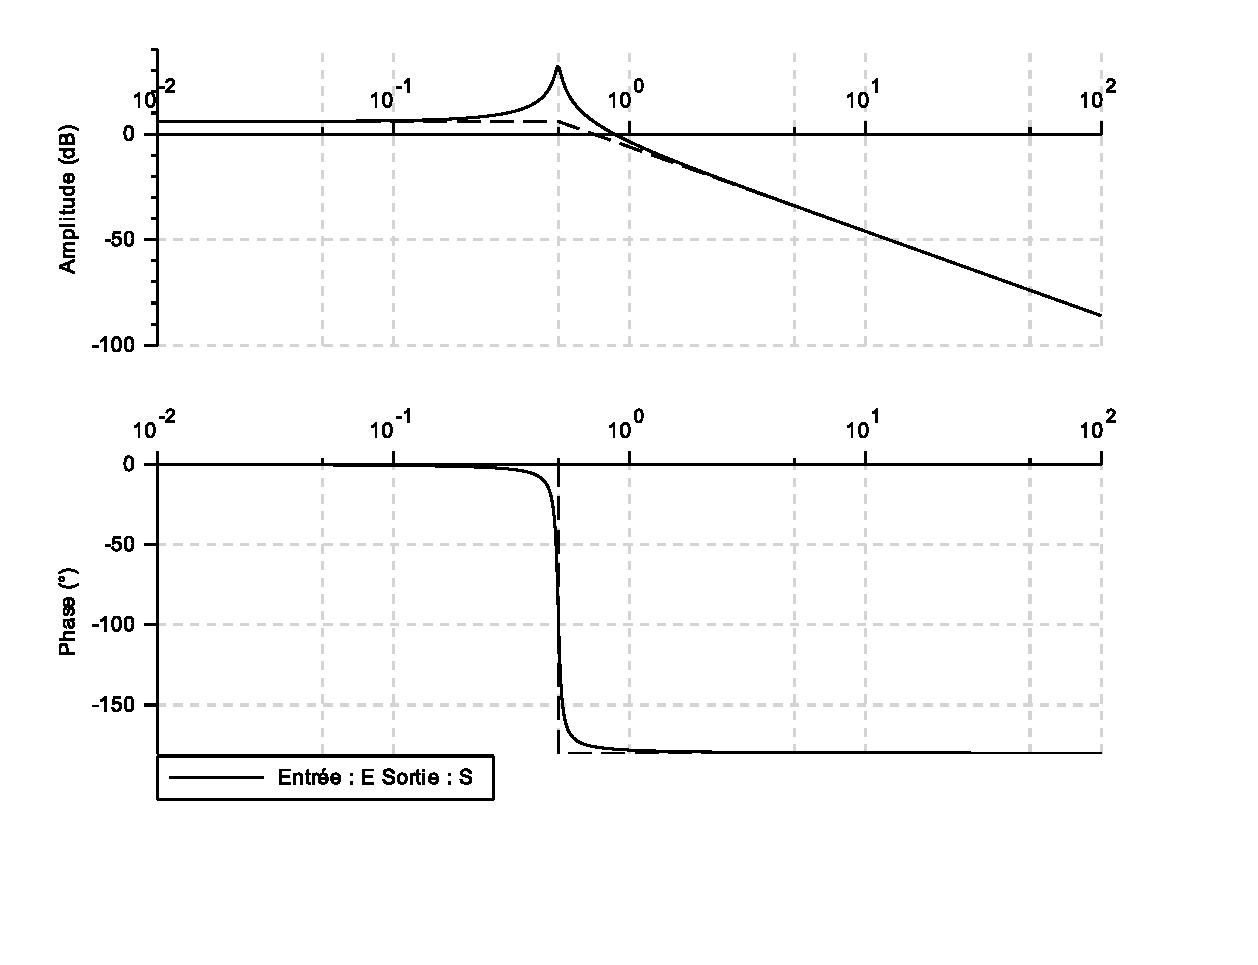
\includegraphics[width=0.8\linewidth]{img/Bode3_c}
\end{center} 

\paragraph{Question 2:} Déterminer la fonction de transfert correspondante.

La tangente à l'infini est de $-40dB/dec$, il s'agit donc d'un second ordre.

La tangente au départ vaut environ $6$, donc $20*log(K)=6$, donc $K\simeq 2$.

Il y a deux cassures, cela signifie que $m>1$.

Les deux cassures sont $\omega_1=10^0=1 rad.s^{-1}$ et $\omega_2=10^2=100 rad.s^{-1}$.

On a donc $\omega_0=\sqrt{\omega_1*\omega_2}=10rad.s^{-1}$ et $z=\dfrac{\omega_0.(\omega_1+\omega_2)}{2.\omega_1.\omega_2}\simeq 5$

La fonction de transfert est donc $H(p)=\dfrac{2}{1+p+0.01*p^2}$.

\newpage

\section{Identification fréquentielle 3}

L'analyse fréquentielle d'un système a donné le tracé suivant.

\paragraph{Question 1:} Tracer les asymptotes à cette courbe.

\begin{center}
 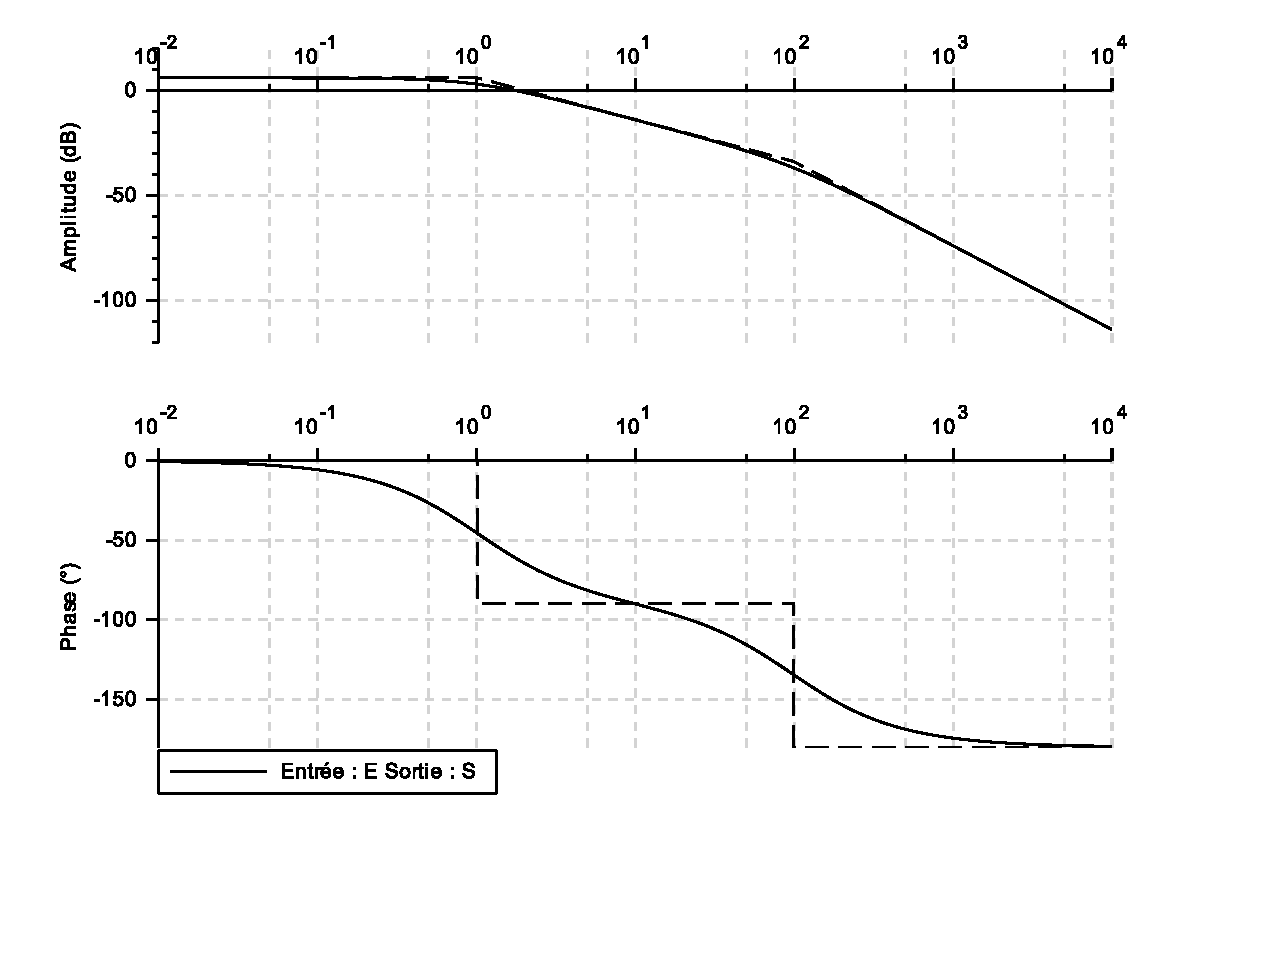
\includegraphics[width=0.8\linewidth]{img/Bode4_c}
\end{center} 

\paragraph{Question 2:} Déterminer la fonction de transfert correspondante.

La tangente à l'infini est de $-40dB/dec$, il s'agit donc d'un second ordre.

La tangente au départ vaut environ $6$, donc $20*log(K)=6$, donc $K\simeq 2$.

La valeur maximale est environ $32$, $20*log(Q)+20*log(K)=32$, donc $20*log(Q)=26$, avec $Q=\dfrac{1}{2.z.\sqrt{1-z^2}}$.

$2.z.\sqrt{1-z^2}=10^{-1.3}$, donc $z\simeq 0.025$.

La pulsation de coupure est $\omega_r=0.5rad.s^{-1}$, avec $\omega_r=\omega_0.\sqrt{1-2.z^2}$, on a ainsi $\omega_0=0.5rad.s^{-1}$.

La fonction de transfert est donc $H(p)=\dfrac{2}{1+0.1*p+4*p^2}$.

\end{document}
